\documentclass[]{article}
\usepackage{amssymb}
\usepackage{amstext}
\usepackage{amsmath}
\usepackage{graphicx} 

\newtheorem{theorem}{Theorem}
\newtheorem{proof}{Proof}
\newtheorem{definition}{Definition}
\newtheorem{claim}{Claim}

%opening
\title{Neural Networks Can Approximate Continuous Functions}
\author{Paul Dubois}
\date{}

\begin{document}

\maketitle

\begin{abstract}
	A clean Tex version of the proof seen during the lectures that neural networks with ReLU activation can approximate continuous functions.
\end{abstract}

\begin{definition}
	$\mathcal{C}\left( \left[ a,b \right] \right)$ is the set of real continuous functions on $\left[ a,b \right]$.
\end{definition}
\begin{definition}
	$\mathcal{P}\left( n,l \right)$ is the set of rectangle 1D-1D perceptrons with $l$ hidden layers and $n$ neurons in each hidden layer.
\end{definition}

\section{Theorem}
$$\forall f \in \mathcal{C}(\left[ a,b \right]), \ \forall \varepsilon > 0, \ \exists N \in \mathbb{N} \text{ and } p \in \mathcal{P}(N,1) \text{ s.t. } \|p-f\|_\infty < \varepsilon$$
Where $\|g\|_\infty$ is infinity norm of $g$ on $\left[ a,b \right]$; i.e. $\|g\|_\infty = \max_{x \in \left[ a,b \right]}(|g(x)|)$.

\section{Idea}
The idea of the proof is to split the interval $\left[ a,b \right]$ in sub intervals such that $f$ has variation less than $\varepsilon$ in the sub-intervals.
Then, choose the weights of the neural network to interpolate linearly $f$ et the beginning and end of the sub-intervals.
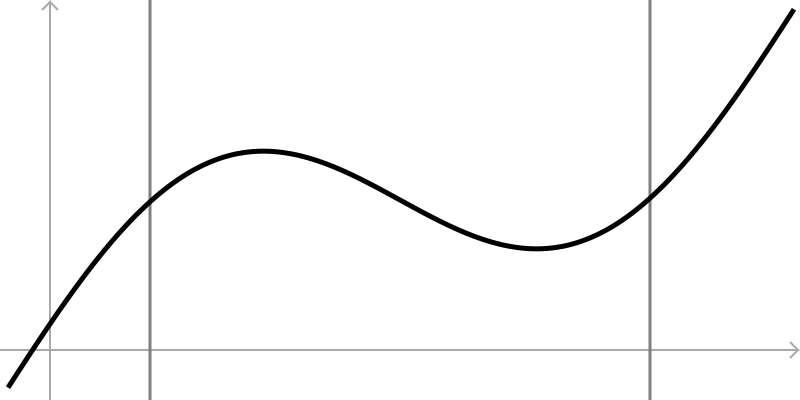
\includegraphics[width=\linewidth]{plot}

\section{Proof}
Let $\varepsilon >0$ and $f \in \mathcal{C}(\left[ a,b \right])$ with $a,b \in \mathbb{R}$, we want $N \in \mathbb{N}$ and $p \in \mathcal{P}(N,1)$ such that $\|p-f\|_\infty < \varepsilon$.

If $p \in \mathcal{P}(N,1)$, then 
$$p(x) = \xi + \sum_{k=0}^{N-1} \gamma_k (\alpha_k x + \beta_k)_+$$
where $(x)_+$ is $\text{ReLU}(x)$.

All we need to do is to find the right coefficients $\xi, \alpha_k, \beta_k, \gamma_k (0 \leq k < N)$ such that $|f(x)-p(x)| < \varepsilon \quad (\forall x \in \left[ a,b \right])$.

Since $f$ is continuous on a compact set, so $f$ is uniformly continuous.
Thus, $\forall x_1,x_2 \in \left[ a,b \right]$, $\exists \delta>0$ such that 
$$|x_1-x_2| < \delta \implies |f(x_1) - f(x_2)| < \varepsilon.$$

Let $c_0 = a$ and $c_{i+1} = c_i + \delta$. Let $N \in \mathbb{N}$ be such that $c_N \geq b$ and redefine $c_N = b$.

\end{document}
